\section{Figures}

\begin{figure}[H]
    \centering
    \caption{True $\mathbb{E}_t\left(r_{t+1}\right)$}
    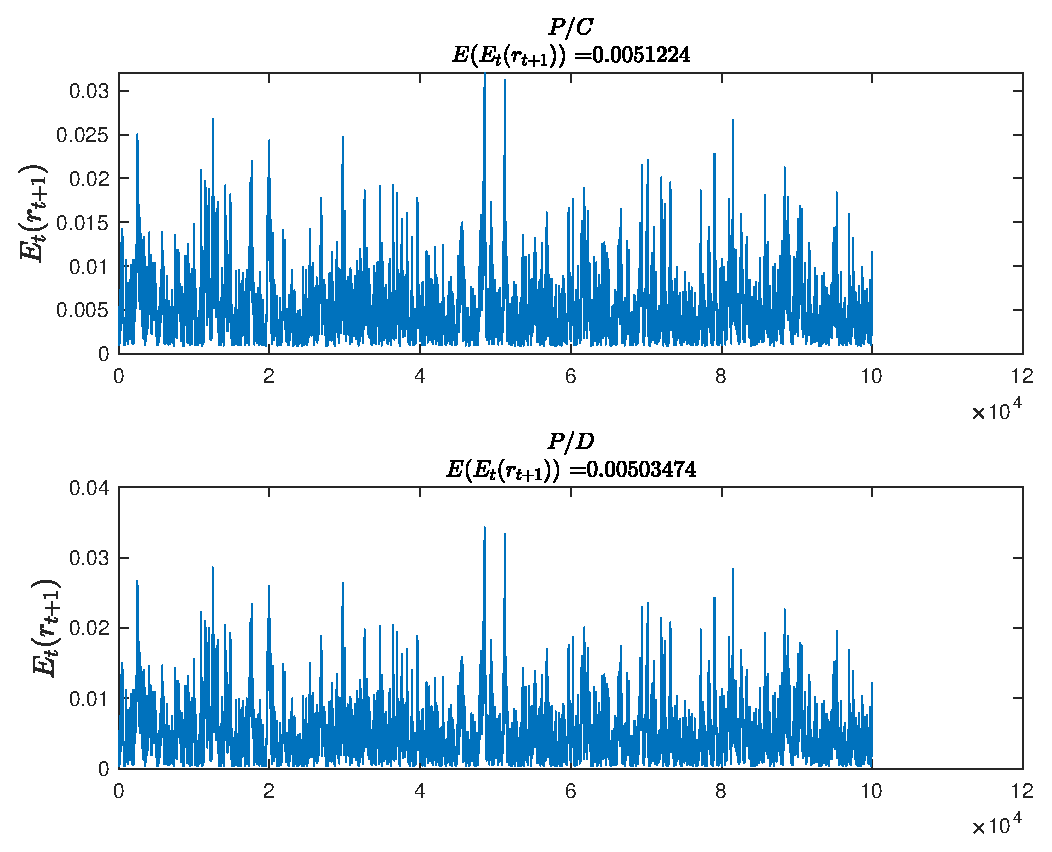
\includegraphics{Figures/Excess_Rets.eps}
    \label{fig:ExpExRets}
\end{figure}
This figure plots the true expected monthly returns of the model. That is for each $t\in\{1,2,...,100.000\}$ the model uses available information up until $t$ to determine the conditional future mean of returns before $t+1$ realizes. 

\begin{figure}[H]
    \centering
    \caption{Chain of simulated annual $P/D$, $P/C$}
    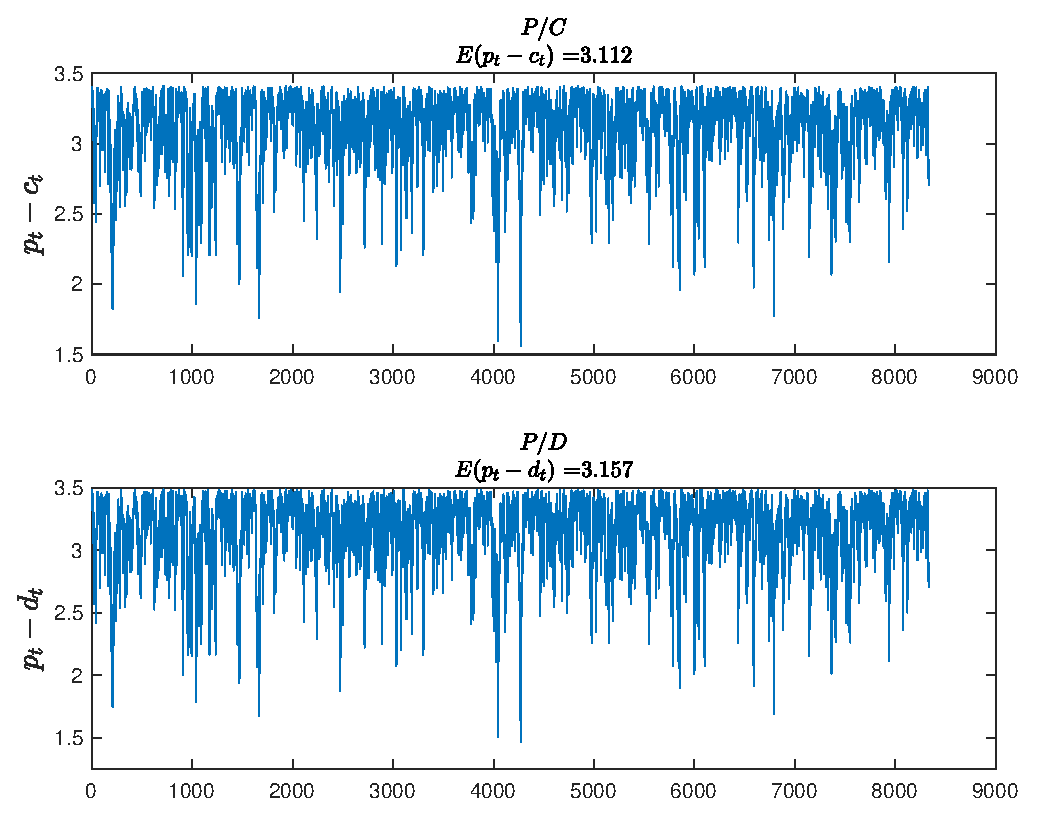
\includegraphics{Figures/PCPD_chain.eps}
    \label{fig:PCPD}
\end{figure}


\section{Code}
\subsection{Main Script and Regressions}
\label{sec:app1}
\lstinputlisting[language=Matlab]{Code_v2/MAIN.m}



\subsection{Functions called by main script}
\label{sec:app2}
\lstinputlisting[language=Matlab]{Code_v2/Functions/mkgrids.m}
\lstinputlisting[language=Matlab]{Code_v2/Functions/findlpc.m}
Note here that an additional file is required! Available here: \url{http://www.holoborodko.com/pavel/numerical-methods/numerical-integration/}\\
This is a \texttt{.mex} file calling a \texttt{c++}-function, greatly increasing the computational efficiency of the integration process
\lstinputlisting[language=Matlab]{Code_v2/Functions/GaussLegendre.m}
\lstinputlisting[language=Matlab]{Code_v2/Functions/pdint.m}
\lstinputlisting[language=Matlab]{Code_v2/Functions/pdmotor.m}
\lstinputlisting[language=Matlab]{Code_v2/Functions/strans.m}
\lstinputlisting[language=Matlab]{Code_v2/Functions/interp.m}
\lstinputlisting[language=Matlab]{Code_v2/Functions/finders.m}
\lstinputlisting[language=Matlab]{Code_v2/Functions/intpcb.m}
\lstinputlisting[language=Matlab]{Code_v2/Functions/intemrs.m}
\lstinputlisting[language=Matlab]{Code_v2/Functions/mrsinsd.m}
\lstinputlisting[language=Matlab]{Code_v2/Functions/inter.m}
\lstinputlisting[language=Matlab]{Code_v2/Functions/erinsd.m}
\lstinputlisting[language=Matlab]{Code_v2/Functions/inter2.m}
\lstinputlisting[language=Matlab]{Code_v2/Functions/interd.m}
\lstinputlisting[language=Matlab]{Code_v2/Functions/erdinsd.m}
\lstinputlisting[language=Matlab]{Code_v2/Functions/inter2d.m}
\lstinputlisting[language=Matlab]{Code_v2/Functions/internorm.m}
\lstinputlisting[language=Matlab]{Code_v2/Functions/erd2ind.m}
\lstinputlisting[language=Matlab]{Code_v2/Functions/intelnr.m}
\lstinputlisting[language=Matlab]{Code_v2/Functions/intelnr2.m}
\lstinputlisting[language=Matlab]{Code_v2/Functions/intelnrcb.m}
\lstinputlisting[language=Matlab]{Code_v2/Functions/ercbin.m}
\lstinputlisting[language=Matlab]{Code_v2/Functions/annvars.m}
\lstinputlisting[language=Matlab]{Code_v2/Functions/chgfreq.m}
\lstinputlisting[language=Matlab]{Code_v2/Functions/simvars.m}
\lstinputlisting[language=Matlab]{Code_v2/Functions/simulacorr.m}
\lstinputlisting[language=Matlab]{Code_v2/Functions/lambda.m}
\lstinputlisting[language=Matlab]{Code_v2/Functions/lambda_Helper.m}
\lstinputlisting[language=Matlab]{Code_v2/Functions/selif.m}
\lstinputlisting[language=Matlab]{Code_v2/Functions/q_s.m}
\lstinputlisting[language=Matlab]{Code_v2/Functions/z_s.m}
\lstinputlisting[language=Matlab]{Code_v2/Functions/nwest.m}
\lstinputlisting[language=Matlab]{Code_v2/Tables/Table_Generator.m}
\lstinputlisting[language=Matlab]{Code_v2/Figures/Figures_CC1998.m}
\lstinputlisting[language=Matlab]{Code_v2/Calibration/Model_Calibration.m}
\begin{comment}
\end{comment}

